\documentclass{article}  % Specifies the document class
\usepackage{amsmath}
\usepackage{ragged2e} % To prevent hyphenation
\usepackage{wrapfig} % Include the wrapfig package
\usepackage{rotating}
\usepackage{graphicx}
\usepackage{tabularx}
\usepackage{biblatex}
\usepackage[margin=1in]{geometry}
\usepackage{fancyhdr}
\usepackage{hyperref}
\usepackage{minted}
\addbibresource{references.bib} % Include your .bib file
\pagestyle{fancy}
\fancyhf{}
\rhead{My Name}
\lhead{Document Title}
\cfoot{\thepage}

\begin{document}         % Begins the document content

\title{My First LaTeX Document}  % Sets the title of the document
\author{Your Name}               % Sets the author of the document
\date{\today}                    % Sets the date (use \today for the current date)

\maketitle                       % Generates the title page

\section{Introduction}           % Creates a section
This is a simple LaTeX document. You can write text here.

\section{Another Section}
You can add more sections and content as needed.

\subsection{A Subsection}
Subsections can also be added.

\begin{table}[h]
\centering
\begin{tabular}{|l|r|}
\hline
\textbf{Left-Aligned} & \textbf{Right-Aligned} \\
\hline
Left text 1 & Right text 1 \\
Left text 2 & Right text 2 \\
Left text 3 & Right text 3 \\
\hline
\end{tabular}
\caption{A simple table with left and right-aligned text.}
\end{table}

\begin{minted}{csharp}
function bubbleSort(arr) {
    let n = arr.length;
    for (let i = 0; i < n - 1; i++) {
        for (let j = 0; j < n - i - 1; j++) {
            if (arr[j] > arr[j + 1]) {
                // Swap without temp variable using addition and subtraction
                arr[j] = arr[j] + arr[j + 1];
                arr[j + 1] = arr[j] - arr[j + 1];
                arr[j] = arr[j] - arr[j + 1];
            }
        }
    }
}

let arr = [64, 34, 25, 12, 22, 11, 90];
bubbleSort(arr);
console.log("Sorted array:", arr);
\end{minted}

% this is a normal table
\begin{table}[h!]
\centering
\begin{tabularx}{\textwidth}{|X|X|X|X|X|X|X|X|X|}
\hline
\textbf{Col 1} & \textbf{Col 2} & \textbf{Col 3} & \textbf{Col 4} & \textbf{Col 5} & \textbf{Col 6} & \textbf{Col 7} & \textbf{Col 8} & \textbf{Col 9} \\
\hline
Data 1 & Data 2 & Data 3 & Data 4 & Data 5 & Data 6 & Data 7 & Data 8 & Data 9 \\
Data 10 & Data 11 & Data 12 & Data 13 & Data 14 & Data 15 & Data 16 & Data 17 & Data 18 \\
Data 19 & Data 20 & Data 21 & Data 22 & Data 23 & Data 24 & Data 25 & Data 26 & Data 27 \\
\hline
\end{tabularx}
\caption{A simple 9-column table.}
\end{table}


\section{Photo Section}
This is a simple LaTeX document with an image included within the text.

Here is an example of including an image:

\begin{wrapfigure}{r}{0.65\textwidth}
    \centering
    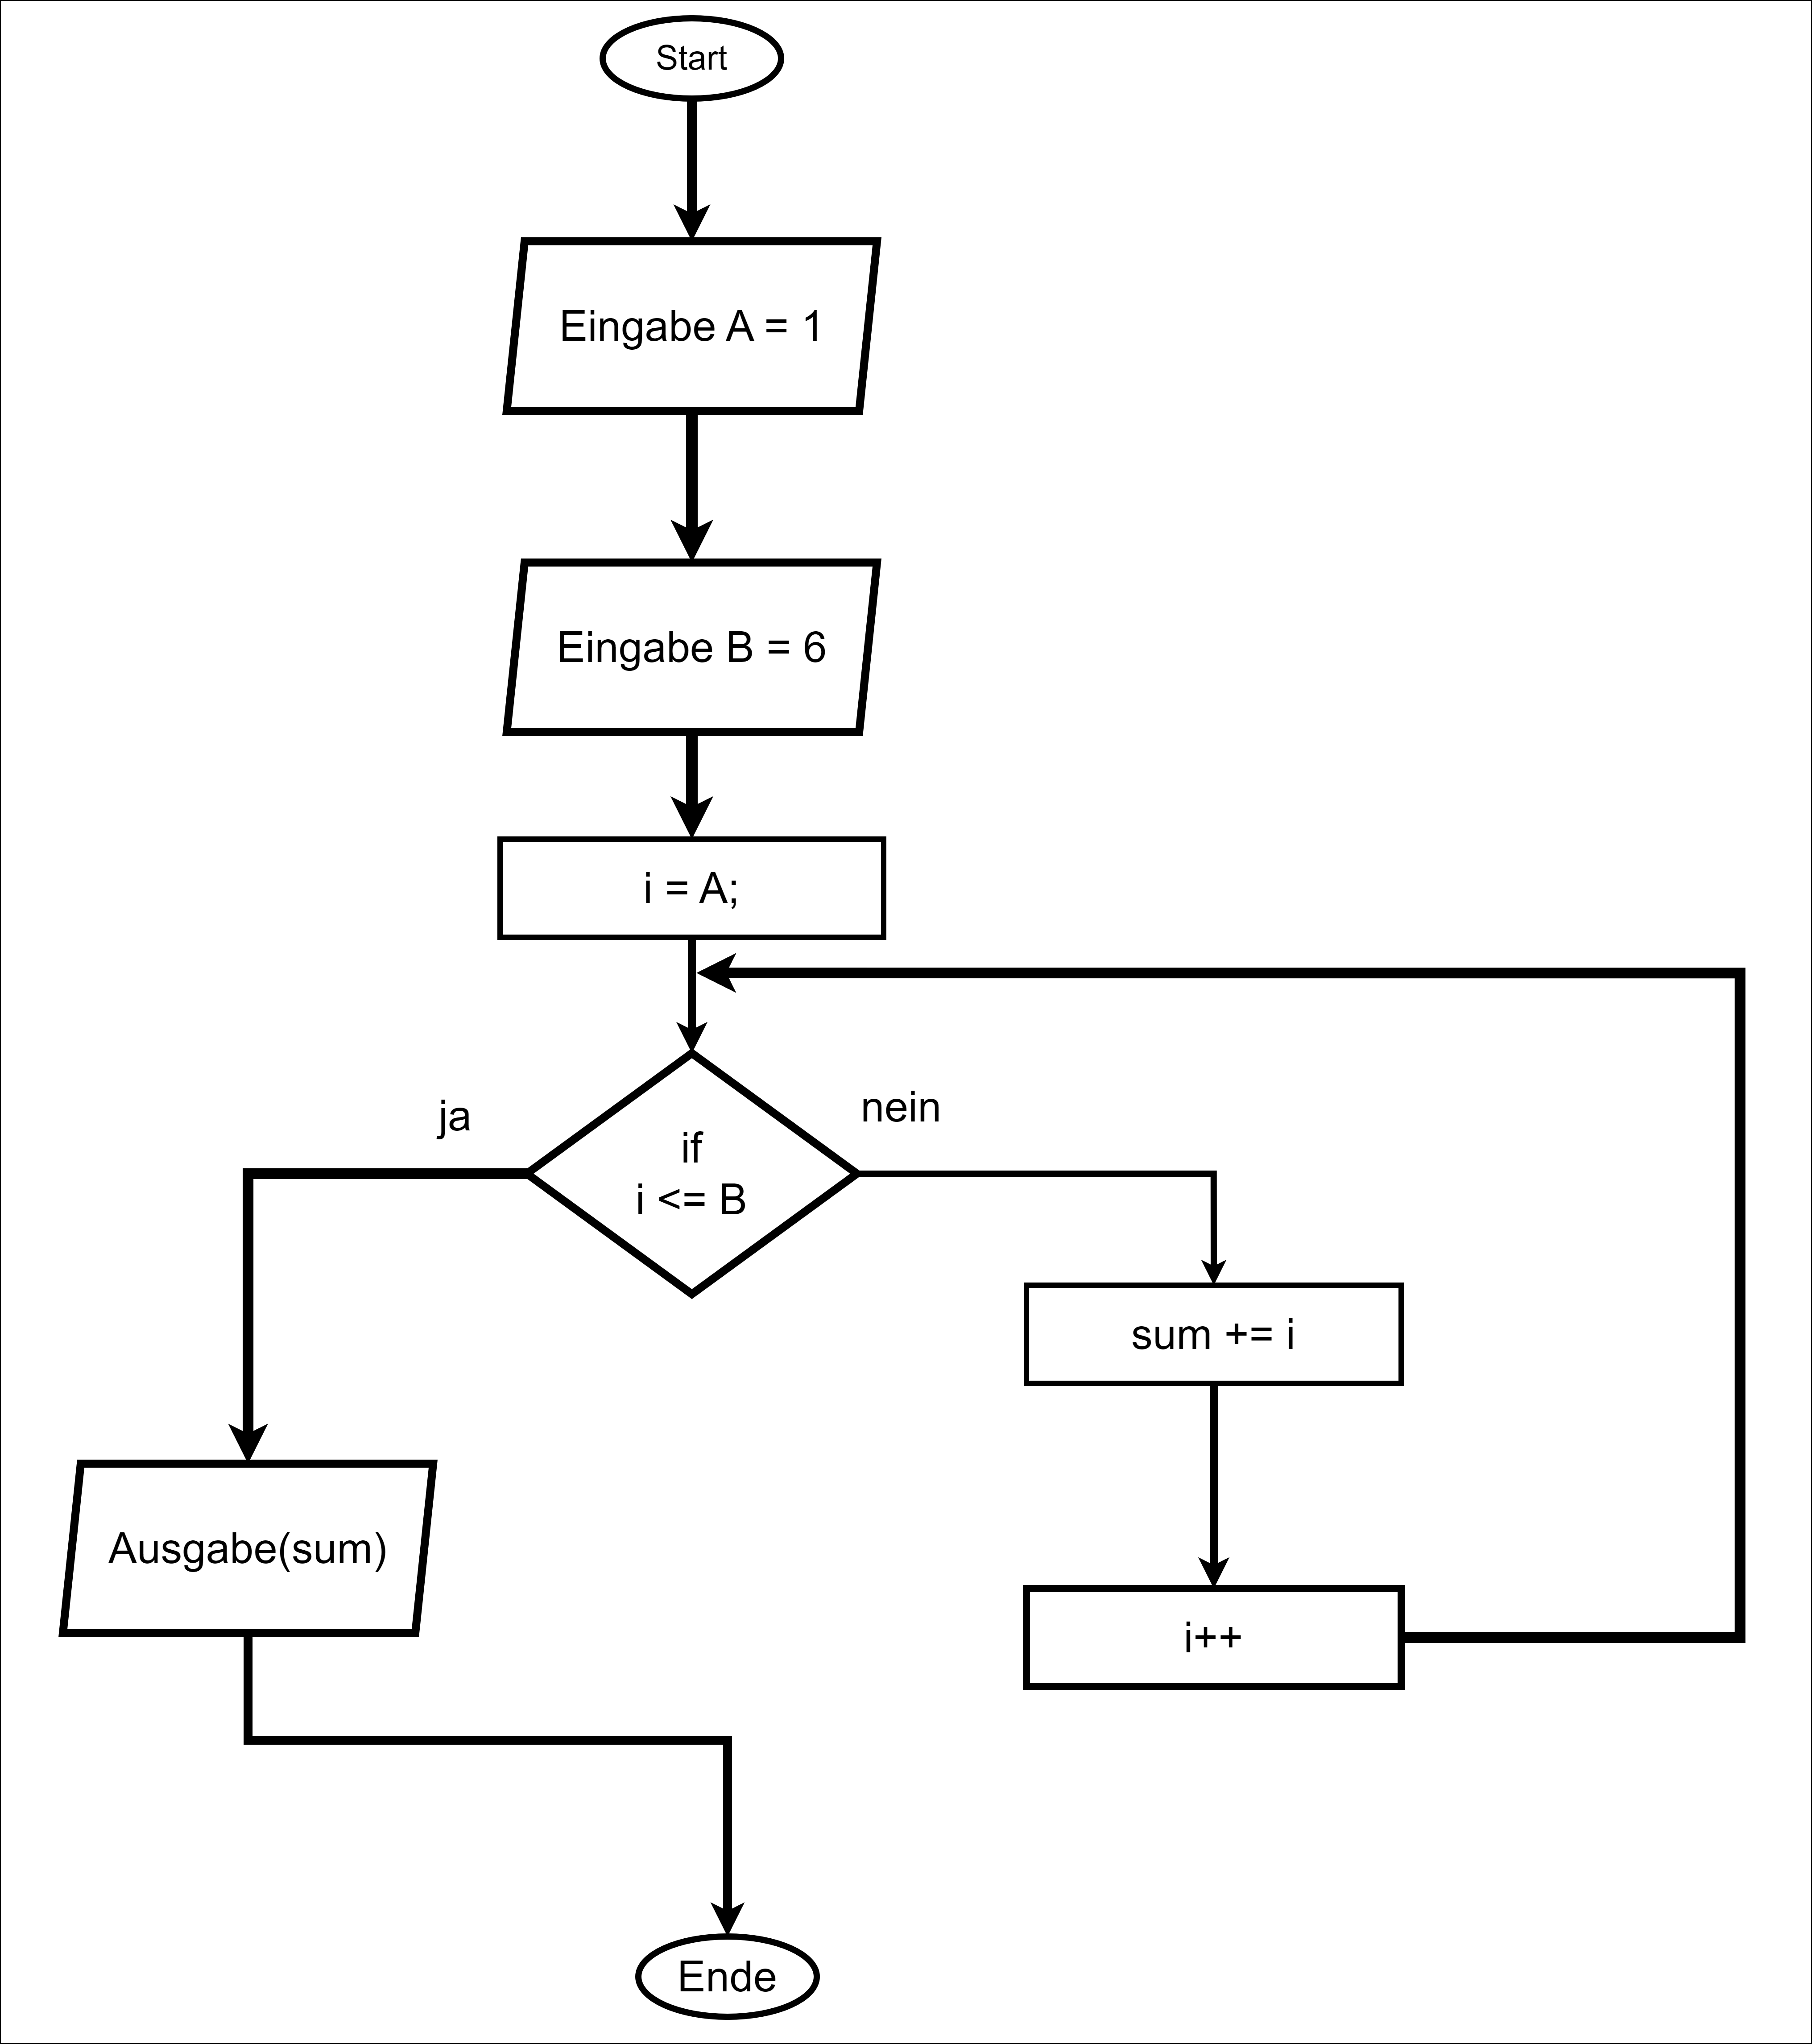
\includegraphics[width=0.60\textwidth]{example-image.png}
    \caption{An example image.}
    \label{fig:example}
\end{wrapfigure}

\begin{justify}
Lorem ipsum dolor sit amet, consectetur adipiscing elit. Nulla varius, massa nec dictum fermentum, erat mauris varius odio, vel cursus augue libero ac nunc. Nam eu est vitae turpis tincidunt vestibulum. Suspendisse potenti. Duis ultrices semper felis, at euismod turpis bibendum vel. Phasellus maximus vehicula nisi, at fermentum augue. Donec facilisis, nisi in fermentum consequat, purus sem convallis sem, a sagittis nisi est ac erat. Curabitur in sagittis lacus, id fringilla leo. Aenean pharetra dui ac metus tempus, at condimentum erat aliquam. Nullam varius, lectus et cursus convallis, sapien metus interdum tortor, nec pellentesque est eros ac odio. Quisque lacinia leo a odio blandit, nec dictum arcu tincidunt. Pellentesque bibendum auctor lacus at sagittis. Vestibulum vestibulum, lectus sed tincidunt fringilla, nisl arcu tincidunt lectus, id tincidunt justo nisi sit amet felis.
Lorem ipsum dolor sit amet, consectetur adipiscing elit. Nulla varius, massa nec dictum fermentum, erat mauris varius odio, vel cursus augue libero ac nunc. Nam eu est vitae turpis tincidunt vestibulum. Suspendisse potenti. Duis ultrices semper felis, at euismod turpis bibendum vel. Phasellus maximus vehicula nisi, at fermentum augue. Donec facilisis, nisi in fermentum consequat, purus sem convallis sem, a sagittis nisi est ac erat. Curabitur in sagittis lacus, id fringilla leo. Aenean pharetra dui ac metus tempus, at condimentum erat aliquam. Nullam varius, lectus et cursus convallis, sapien metus interdum tortor, nec pellentesque est eros ac odio. Quisque lacinia leo a odio blandit, nec dictum arcu tincidunt. Pellentesque bibendum auctor lacus at sagittis. Vestibulum vestibulum, lectus sed tincidunt fringilla, nisl arcu tincidunt lectus, id tincidunt justo nisi sit amet felis.
\end{justify}

As shown in Figure \ref{fig:example}, the image is centered and scaled to half the text width.

\section{Photo Section with cm}
This is a simple LaTeX document with an image included within the text.

Here is an example of including an image:

\begin{wrapfigure}{r}{8cm} % Adjust the width as needed
    \centering
    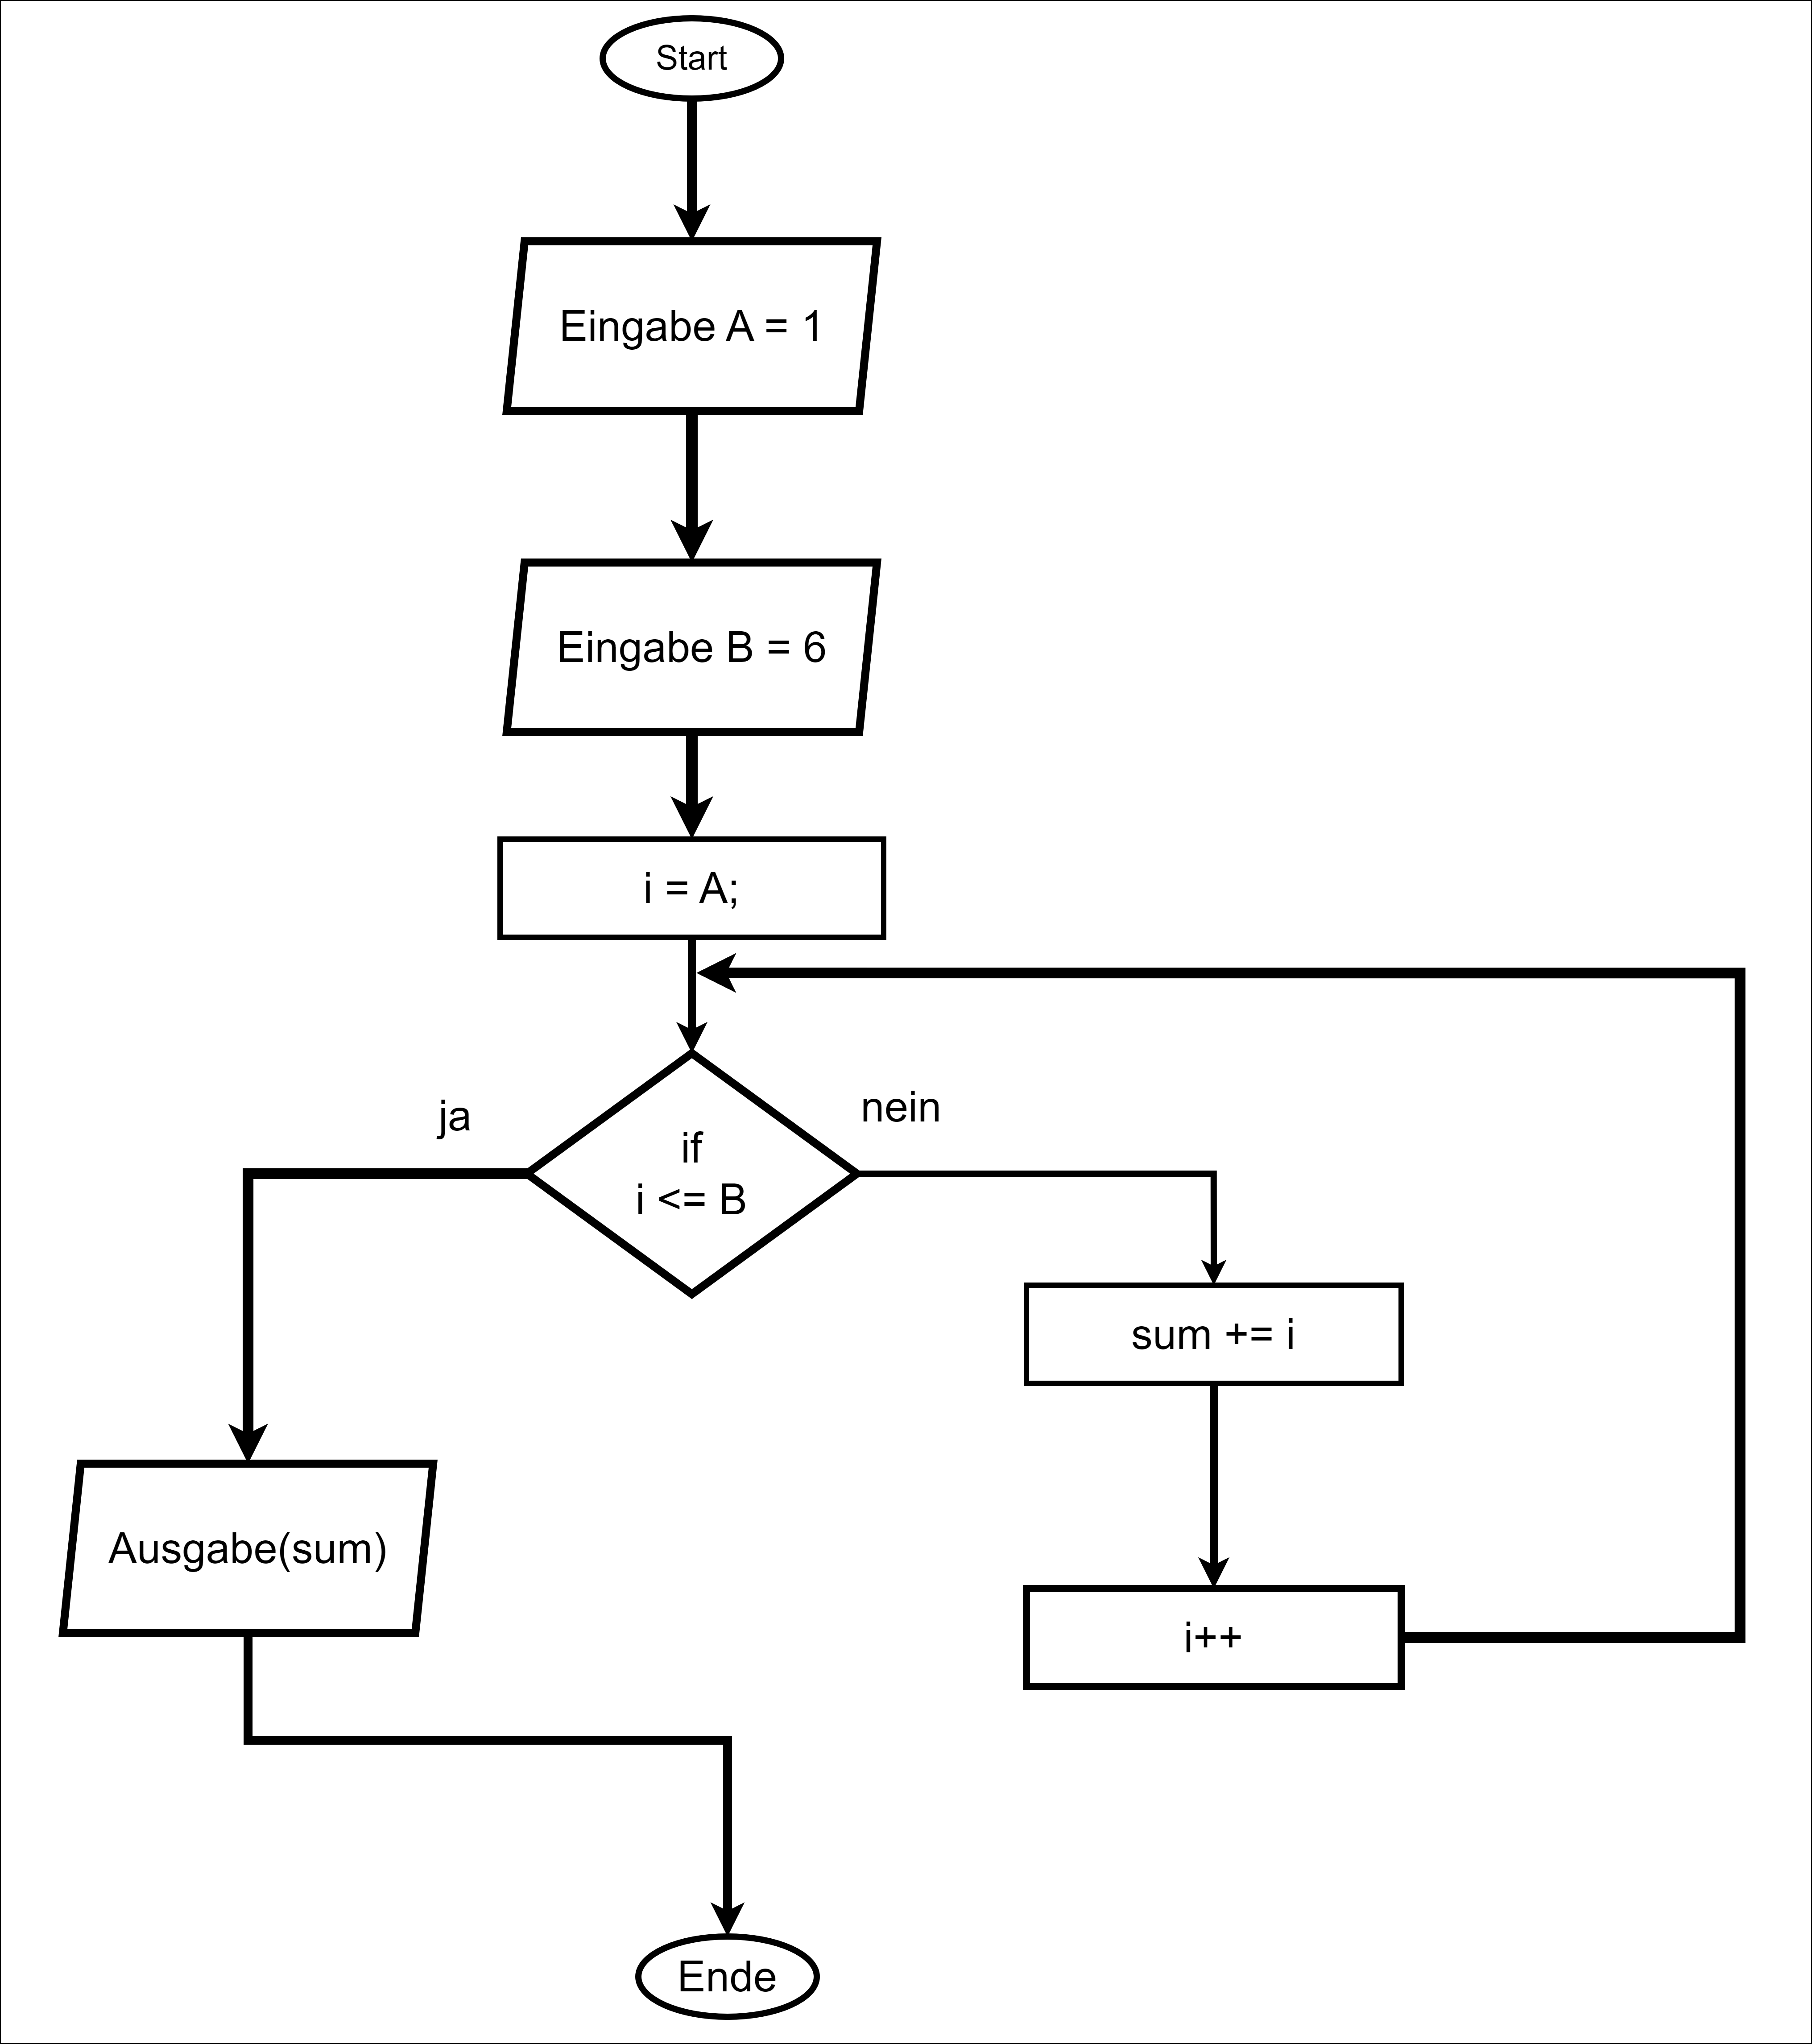
\includegraphics[width=7.8cm]{example-image.png} % Adjust the width slightly less than wrapfigure width
    \caption{An example image.}
    \label{fig:example}
\end{wrapfigure}

\begin{justify}
Lorem ipsum dolor sit amet, consectetur adipiscing elit. Nulla varius, massa nec dictum fermentum, erat mauris varius odio, vel cursus augue libero ac nunc. Nam eu est vitae turpis tincidunt vestibulum. Suspendisse potenti. Duis ultrices semper felis, at euismod turpis bibendum vel. Phasellus maximus vehicula nisi, at fermentum augue. Donec facilisis, nisi in fermentum consequat, purus sem convallis sem, a sagittis nisi est ac erat. Curabitur in sagittis lacus, id fringilla leo. Aenean pharetra dui ac metus tempus, at condimentum erat aliquam. Nullam varius, lectus et cursus convallis, sapien metus interdum tortor, nec pellentesque est eros ac odio. Quisque lacinia leo a odio blandit, nec dictum arcu tincidunt. Pellentesque bibendum auctor lacus at sagittis. Vestibulum vestibulum, lectus sed tincidunt fringilla, nisl arcu tincidunt lectus, id tincidunt justo nisi sit amet felis.
Lorem ipsum dolor sit amet, consectetur adipiscing elit. Nulla varius, massa nec dictum fermentum, erat mauris varius odio, vel cursus augue libero ac nunc. Nam eu est vitae turpis tincidunt vestibulum. Suspendisse potenti. Duis ultrices semper felis, at euismod turpis bibendum vel. Phasellus maximus vehicula nisi, at fermentum augue. Donec facilisis, nisi in fermentum consequat, purus sem convallis sem, a sagittis nisi est ac erat. Curabitur in sagittis lacus, id fringilla leo. Aenean pharetra dui ac metus tempus, at condimentum erat aliquam. Nullam varius, lectus et cursus convallis, sapien metus interdum tortor, nec pellentesque est eros ac odio. Quisque lacinia leo a odio blandit, nec dictum arcu tincidunt. Pellentesque bibendum auctor lacus at sagittis. Vestibulum vestibulum, lectus sed tincidunt fringilla, nisl arcu tincidunt lectus, id tincidunt justo nisi sit amet felis.
Lorem ipsum dolor sit amet, consectetur adipiscing elit. Nulla varius, massa nec dictum fermentum, erat mauris varius odio, vel cursus augue libero ac nunc. Nam eu est vitae turpis tincidunt vestibulum. Suspendisse potenti. Duis ultrices semper felis, at euismod turpis bibendum vel. Phasellus maximus vehicula nisi, at fermentum augue. Donec facilisis, nisi in fermentum consequat, purus sem convallis sem, a sagittis nisi est ac erat. Curabitur in sagittis lacus, id fringilla leo. Aenean pharetra dui ac metus tempus, at condimentum erat aliquam. Nullam varius, lectus et cursus convallis, sapien metus interdum tortor, nec pellentesque est eros ac odio. Quisque lacinia leo a odio blandit, nec dictum arcu tincidunt. Pellentesque bibendum auctor lacus at sagittis. Vestibulum vestibulum, lectus sed tincidunt fringilla, nisl arcu tincidunt lectus, id tincidunt justo nisi sit amet felis.
\end{justify}

% this is a horizontal table
\begin{sidewaystable}
\centering
\resizebox{\textwidth}{!}{%
\begin{tabular}{|l|c|r|l|l|c|c|r|r|}
\hline
\textbf{Left-Aligned} & \textbf{Center-Aligned} & \textbf{Right-Aligned} & \textbf{Left-Aligned} & \textbf{Left-Aligned} & \textbf{Center-Aligned} & \textbf{Right-Aligned} & \textbf{Left-Aligned} & \textbf{Left-Aligned} \\
\hline
Left text 1 & Center text 1 & Right text 1 & Left text 1 & Left text 1 & Center text 1 & Right text 1 & Left text 1 & Left text 1 and even more words here and even more stuff here!!! and even more text here!\\
Left text 2 & Center text 2 & Right text 2 & Left text 2 & Left text 2 & Center text 2 & Right text 2 & Left text 2 & Left text 2 \\
Left text 3 & Center text 3 & Right text 3 & Left text 3 & Left text 3 & Center text 3 & Right text 3 & Left text 3 & Left text 3 \\
Left text 4 & Center text 4 & Right text 4 & Left text 4 & Left text 4 & Center text 4 & Right text 4 & Left text 4 & Left text 4 \\
Left text 5 & Center text 5 & Right text 5 & Left text 5 & Left text 5 & Center text 5 & Right text 5 & Left text 5 & Left text 5 \\
Left text 6 & Center text 6 & Right text 6 & Left text 6 & Left text 6 & Center text 6 & Right text 6 & Left text 6 & Left text 6 \\
Left text 7 & Center text 7 & Right text 7 & Left text 7 & Left text 7 & Center text 7 & Right text 7 & Left text 7 & Left text 7 \\
Left text 8 & Center text 8 & Right text 8 & Left text 8 & Left text 8 & Center text 8 & Right text 8 & Left text 8 & Left text 8 \\
Left text 9 & Center text 9 & Right text 9 & Left text 9 & Left text 9 & Center text 9 & Right text 9 & Left text 9 & Left text 9 \\
Left text 10 & Center text 10 & Right text 10 & Left text 10 & Left text 10 & Center text 10 & Right text 10 & Left text 10 & Left text 10 \\
Left text 11 & Center text 11 & Right text 11 & Left text 11 & Left text 11 & Center text 11 & Right text 11 & Left text 11 & Left text 11 \\
Left text 12 & Center text 12 & Right text 12 & Left text 12 & Left text 12 & Center text 12 & Right text 12 & Left text 12 & Left text 12 \\
Left text 13 & Center text 13 & Right text 13 & Left text 13 & Left text 13 & Center text 13 & Right text 13 & Left text 13 & Left text 13 \\
Left text 14 & Center text 14 & Right text 14 & Left text 14 & Left text 14 & Center text 14 & Right text 14 & Left text 14 & Left text 14 \\
Left text 15 & Center text 15 & Right text 15 & Left text 15 & Left text 15 & Center text 15 & Right text 15 & Left text 15 & Left text 15 \\
Left text 16 & Center text 16 & Right text 16 & Left text 16 & Left text 16 & Center text 16 & Right text 16 & Left text 16 & Left text 16 \\
Left text 17 & Center text 17 & Right text 17 & Left text 17 & Left text 17 & Center text 17 & Right text 17 & Left text 17 & Left text 17 \\
Left text 18 & Center text 18 & Right text 18 & Left text 18 & Left text 18 & Center text 18 & Right text 18 & Left text 18 & Left text 18 \\
Left text 19 & Center text 19 & Right text 19 & Left text 19 & Left text 19 & Center text 19 & Right text 19 & Left text 19 & Left text 19 \\
Left text 20 & Center text 20 & Right text 20 & Left text 20 & Left text 20 & Center text 20 & Right text 20 & Left text 20 & Left text 20 \\
\hline
\end{tabular}
}
\caption{A table with left, center, and right-aligned text.}
\end{sidewaystable}

\end{document}         % Ends the document content
